\section{The Problem: What Breaks, When, and For Whom}\label{sec:problem}

\subsection{The immediate problem (2026--2027): the price of not knowing your own number}

Take a representative Gangshan SME shipping standard carbon-steel fasteners
($\sim$2~tCO$_2$e embedded per tonne of product\cite{specialinsert}). At the
official EUR~75.3 certificate price\cite{ecprice}, its EU buyer pays about
\textbf{EUR~150 per tonne} of fasteners --- \emph{if the factory supplies
verified data}. If it cannot, the buyer falls back on default values that
industry analysts estimate at 3--5 times the verified cost, escalating each
year (Figure~\ref{fig:cbamcost}). Against sector-average export prices near
US\$3,400--3,600 per tonne --- and far less for commodity lines --- analysts
put worst-case default exposure as high as \textbf{30--50\% of product
value}\cite{specialinsert}.

\begin{figure}[htbp]
\centering
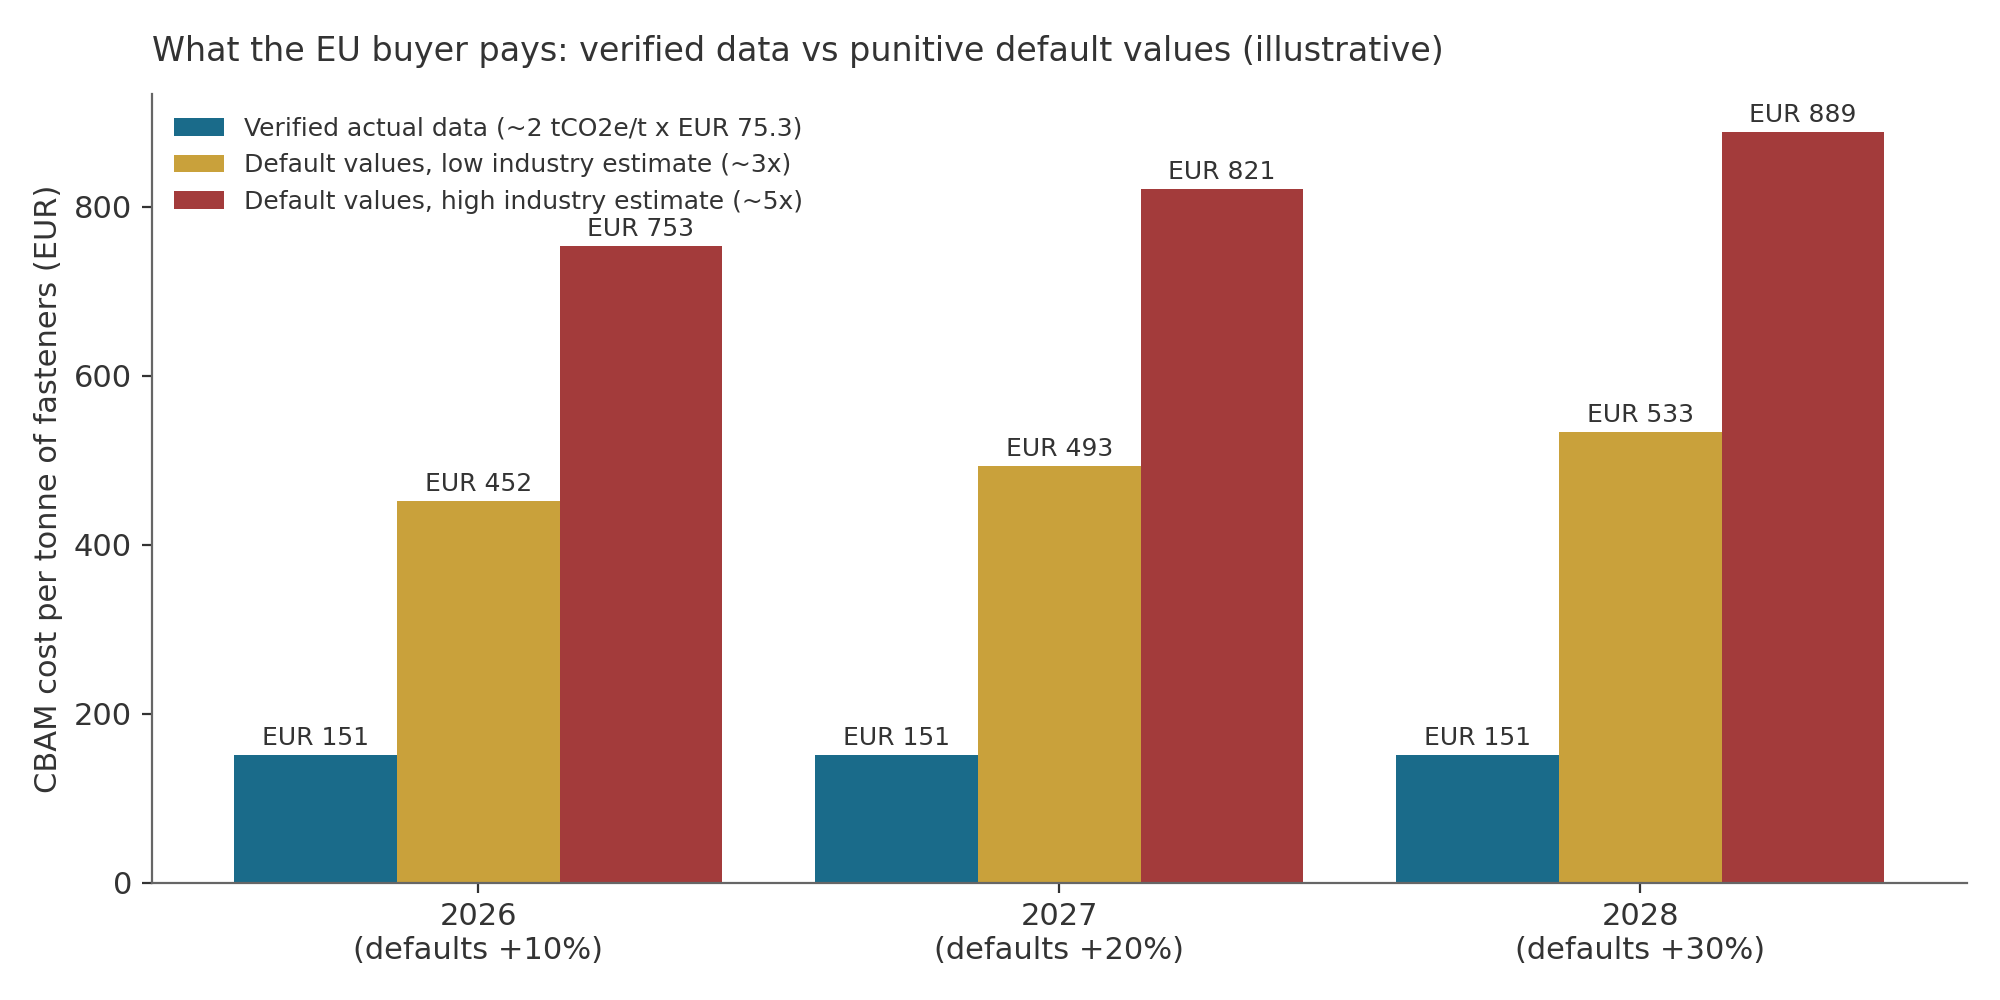
\includegraphics[width=0.95\textwidth]{chart3_cbam.png}
\caption[CBAM cost per tonne: verified data vs.\ default values]{Illustrative
CBAM cost per tonne of fasteners at the official EUR~75.3/tCO$_2$e certificate
price\cite{ecprice}, comparing verified actual data ($\sim$2
tCO$_2$e/t\cite{specialinsert}) with low and high industry estimates of
default-value multiples, escalated by the regulation's markup
schedule\cite{omm}.}
\label{fig:cbamcost}
\end{figure}

\begin{keyfact}{Why even tiny suppliers get caught.}
The 50-tonne exemption is counted per EU importer, across all its suppliers
combined. MOENV's Climate Change Administration Director-General publicly
warned of the consequence: a European distributor buying ten tonnes each from
five Taiwanese SMEs crosses the threshold --- and must then demand verified
data from all five\cite{tpt-cbam}. The smallest factory in Gangshan can inherit
a European compliance obligation it has never heard of.
\end{keyfact}

The commercial logic is brutal and impersonal: an importer facing two otherwise
identical Taiwanese suppliers keeps the one whose data pack arrives with the
shipment. And the capability to respond is demonstrably thin: sector surveys
found \textbf{60\%} of fast-growing SMEs had completed no carbon inventory,
\textbf{80\%} had no reduction targets, and half cited talent shortage as the
binding constraint\cite{cw}. A handful of cluster firms (e.g., Chan Chin C.,
Fang Sheng) have obtained ISO~14067 product-footprint certificates through
subsidized counseling\cite{chanchin} --- proof the task is \emph{tractable},
and proof of the economics problem: consultant-priced, one-off snapshots cannot
serve recurring, per-product, per-quarter data demands across 2,600 firms.

\subsection{The compounding problem (2027--2030): four ratchets}

\begin{table}[htbp]
\caption{The cost of doing nothing, year by year}
\label{tab:ratchets}
\small
\begin{tabularx}{\textwidth}{@{}p{0.16\textwidth}Xp{0.3\textwidth}@{}}
\toprule
\textbf{Ratchet} & \textbf{Mechanism} & \textbf{Effect on a Gangshan SME} \\
\midrule
Default markup & +10\% (2026) $\to$ +20\% (2027) $\to$ +30\% (2028), automatic\cite{omm} & The penalty for having no data rises every year without anyone lifting a finger \\
Scope extension & $\sim$180 downstream steel/aluminium categories proposed; obligations from 2028 if passed (EP vote Sep 2026)\cite{akin} & Neighbours making springs, wire, hand tools join the same regime \\
Product passports & EU Digital Product Passport registry launches Jul 2026; batteries mandatory 2027; steel, textiles, electronics phased 2027--2030\cite{espr} & Product-level, machine-readable sustainability data becomes a condition of EU market access \\
Domestic expansion & Fee threshold lowering; rates rising toward NT\$1,200--1,800/t by 2030; ETS pilot $\sim$2027\cite{ecobiz} & Firms outside the carbon fee today are progressively pulled inside it \\
\bottomrule
\end{tabularx}
\end{table}

In 2024, a fastener maker's carbon ignorance cost it nothing. In 2026 it costs
its buyer several hundred euros per tonne and puts the relationship at risk. By
2028 the penalty is a third higher, the covered catalogue potentially far
larger, and Taiwan's own regulator closer to the factory gate. \textbf{The
problem is not a wave; it is a rising floor.}

\section{The Gap: Why Nothing in the Current System Solves This}\label{sec:gap}

Taiwan's government has not been idle --- it has built an entire
\emph{awareness} stack. What no instrument does is produce the artifact that
decides procurement outcomes: verified-ready, per-product embedded-emissions
data in the European Commission's format. Table~\ref{tab:gap} is a capability
audit of everything that exists, verified as of July 2026.

\begin{table}[htbp]
\caption{Capability audit of existing instruments}
\label{tab:gap}
\small
\begin{tabularx}{\textwidth}{@{}p{0.26\textwidth}p{0.33\textwidth}X@{}}
\toprule
\textbf{Instrument} & \textbf{What it does} & \textbf{What it does not do} \\
\midrule
CAAS ``SME Carbon Reduction Service Station'' (MOEA)\cite{caas} & Courses, articles, green-product promotion, consultant referrals & No computation of any kind; not a reporting tool \\
IDB Carbon Emissions Calculator (MOEA)\cite{idb} & Free web tool: bills + fuel lists $\to$ rough annual company-level CO$_2$e & No product-level allocation, no CN-code output, no CBAM format \\
MOENV CBAM Help Platform (Mar 2026)\cite{tpt-cbam} & Information hub and consultation channel for affected SMEs & Explicitly informational; computes nothing \\
Taipower app / eBill\cite{taipower} & Consumption charts, tariff simulation, usage alerts for smart-meter customers & No emissions conversion; no compliance artifacts \\
tre100 (CIER, Dec 2025)\cite{tre100} & Renewable-electricity pledge registry below RE100's threshold & No measurement tooling, no accounting \\
Private ESG software + consultants\cite{chanchin} & Organizational inventories; real ISO certifications via subsidized counseling & Per-engagement pricing; recurring per-product CBAM packs remain manual, unaffordable at micro-SME scale \\
\bottomrule
\end{tabularx}
\end{table}

\textbf{The gap, stated precisely:} no instrument converts \emph{SME-native
documents} --- a Taipower bill, a stack of invoices, a production ledger ---
into \emph{importer-ready, verifier-structured, per-CN-code emissions data},
repeatably and at near-zero marginal cost. The government stack ends at
awareness; the market stack prices out the small end. And because MOENV has
already built the informational front door\cite{tpt-cbam}, a computational
layer designed for integration \emph{completes} a stack the state has visibly
started building.
